\section{Lagrange Enters: The Death of Geometry, the Rise of Symmetry (1788)}



\subsection*{The Lagrangian Method: Mechanics Without Diagrams}


Euler had fused calculus and mechanics. But even he still leaned on geometry when dealing with planetary motion. Then came \textbf{Joseph-Louis Lagrange}, and with him, the final blow to triangles, diagrams, and classical constructions.

\begin{quote}
\textit{"Mechanics ought to be treated like algebra."}
\end{quote}

Lagrange’s key insight was to describe the motion of a system not through forces or figures, but through a symbolic function—what he called the \textit{formula of living forces diminished by the potential forces}. In modern language:

\[
L = T - V
\]

But Lagrange expressed this without explicit vector notation or partial derivatives. His formulation was built entirely on:
\begin{itemize}
    \item Generalized coordinates \( q_1, q_2, \ldots \)
    \item Velocities \( \frac{dq_1}{dt}, \frac{dq_2}{dt}, \ldots \)
    \item Ordinary differentials, not partials
\end{itemize}

To describe motion, Lagrange summed kinetic and potential energy symbolically. His core principle was this: 

\begin{quote}
the actual path of a system makes the quantity \( L \) yield a stationary value under infinitesimal variations of the \( q_i \). 
\end{quote}

This principle of \textit{virtual velocities} produced what we now call the Euler-Lagrange equation, though Lagrange wrote it as:

\[
\frac{d}{dt} \left( \frac{dL}{d\dot{q}_i} \right) - \frac{dL}{dq_i} = 0
\]

where \( \dot{q}_i \) was simply shorthand for \( \frac{dq_i}{dt} \), and the derivatives \( \frac{dL}{dq_i} \) were taken as total differentials with respect to each coordinate.

\subsection*{Kepler’s Second Law Emerges — Without a Word About Kepler}

In the case of planetary motion, Lagrange considered two coordinates: one for the radial distance from the sun, and one for the angular position along the orbit. He did not name them \( r \) or \( \theta \), but represented them abstractly as \( q_1 \) and \( q_2 \).

The kinetic energy, expressed in Lagrange's form, would be something like:

\[
T = \frac{1}{2} m \left( \left( \frac{dq_1}{dt} \right)^2 + a(q_1)^2 \left( \frac{dq_2}{dt} \right)^2 \right)
\]

Here:
\begin{itemize}
    \item \( q_1 \) denotes the radial distance
    \item \( q_2 \) denotes the angular position
    \item \( a(q_1) \) represents a generalized arm or rotational arc-length function
\end{itemize}

Lagrange observed: if a coordinate like \( q_2 \) does not appear explicitly in the expression for \( L \), then the quantity associated with its "velocity" \( \frac{dq_2}{dt} \) remains constant over time.

\[
\frac{dL}{dq_2} = 0 \quad \Rightarrow \quad \frac{d}{dt} \left( \frac{dL}{d\dot{q}_2} \right) = 0
\]

Thus, the product \( a(q_1)^2 \cdot \frac{dq_2}{dt} \) is constant — which is equivalent to the conservation of angular momentum. This is precisely the mathematical structure behind Kepler’s Second Law: that a planet sweeps out equal areas in equal times.

But Lagrange never needed to say it. It simply fell out of the algebra.

\subsubsection*{Conservation Laws from Lagrangian Symmetry}

Lagrange's framework made conservation a matter of structure. Instead of relying on geometric intuition, his method revealed which physical quantities stay constant—based on the symmetries of the system.

\begin{center}
\renewcommand{\arraystretch}{1.5}
\begin{tabular}{|c|l|l|}
\hline
\textbf{Symmetry in L} & \textbf{What It Means} & \textbf{What’s Conserved} \\ \hline
\( q_i \) not in \( L \) & The coordinate doesn't appear explicitly & Momentum conjugate to \( q_i \) \\ \hline
\( L \) has no \( t \) & The system is time-invariant & Total energy (Hamiltonian) \\ \hline
No angular coordinate in \( L \) & The system is rotationally symmetric & Angular momentum \(\Rightarrow\) Equal areas swept \\ \hline
\end{tabular}
\end{center}

\begin{quote}
\textit{Lagrange didn’t prove Kepler’s law. He absorbed it.}
\end{quote}

\vspace{1em}

\subsection*{Lagrange’s Power Move: The Summary Table}

\begin{center}
\renewcommand{\arraystretch}{1.5}
\begin{tabular}{|c|l|}
\hline
\textbf{Mathematician} & \textbf{How They Treated Kepler’s Second Law} \\ \hline
\textbf{Newton} & Proved it geometrically using triangles and central forces \\ \hline
\textbf{Euler} & Explained it as the conservation of rotational resistance (inertia) \\ \hline
\textbf{Lagrange} & Derived it from symmetry in equations—no mention of orbits required \\ \hline
\end{tabular}
\end{center}

\vspace{0.5em}

Lagrange’s mechanics was blind to shapes and curves.  
It saw only structure—and conserved what mattered.

\subsection*{Diagram: Lagrangian Coordinates and Symmetry}

The following diagram represents a Lagrangian approach to planetary motion. It avoids modern vector or polar notation and instead shows generalized coordinates \( q_1 \) and \( q_2 \), where:

\begin{itemize}
    \item \boldmath\( q_1 \): \unboldmath This coordinate represents the radial distance from the central body — such as the Sun in a planetary system. It tells us how far the orbiting body (e.g., a planet or comet) is at any moment. Unlike Cartesian coordinates that break space into rigid gridlines, \( q_1 \) captures the natural symmetry of gravitational motion: what's most important is how far the object is from the center of attraction, not where it is on an \( x \)-\( y \) plane. This makes \( q_1 \) a physically intuitive choice when modeling motion governed by central forces.

    \item \boldmath\( q_2 \): \unboldmath This is an abstract angular coordinate — it plays the role of "sweeping out" direction, but it’s not necessarily labeled \( \theta \) or tied to standard polar coordinates. In Lagrangian mechanics, we’re allowed to pick generalized coordinates that best exploit the symmetry of the system. Here, \( q_2 \) tracks how the body moves around the center, but what’s most important is that the Lagrangian doesn’t explicitly depend on \( q_2 \) itself — only on how fast \( q_2 \) is changing. That absence hints at a deeper symmetry: the system looks the same no matter what the current value of \( q_2 \) is. This rotational symmetry is the key to conservation of angular momentum.

    \item \boldmath\( L(q_1, q_2, \dot{q}_1, \dot{q}_2) \): \unboldmath The Lagrangian is a function that encodes the dynamics of the system — it typically takes the form of "kinetic energy minus potential energy." In this case, the Lagrangian depends on the position and velocity in both radial and angular directions. However, if it contains no explicit dependence on \( q_2 \), then a powerful result from Lagrangian mechanics (via Noether’s theorem) tells us that the derivative \( \frac{dL}{d\dot{q}_2} \) is conserved. This quantity is known as the \textbf{conjugate momentum} to \( q_2 \), and in physical terms, it corresponds to \textbf{angular momentum}.

    This conservation law is not a coincidence — it is a direct reflection of the rotational symmetry of the system. If rotating the entire configuration by some angle doesn’t change the physics, then angular momentum must be conserved. This is the modern mathematical expression of \textit{Kepler’s Second Law} — that equal areas are swept out in equal times.
\end{itemize}


\begin{figure}[H]
\centering
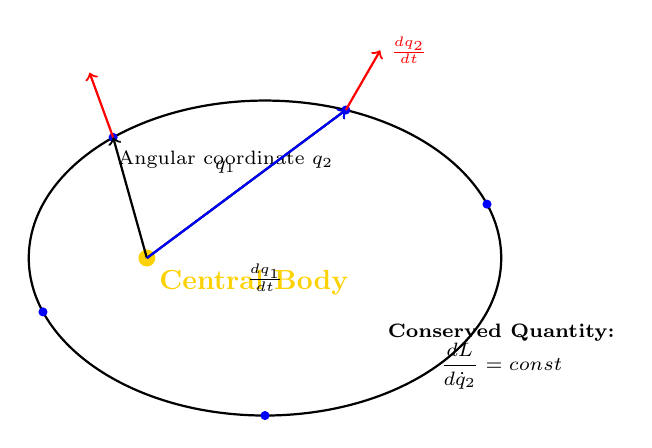
\begin{tikzpicture}[scale=2.5]

  % Draw the orbit path (elliptical trajectory)
  \draw[thick] (0,0) ellipse (1.2 and 0.8);

  % Central body (e.g., Sun)
  \filldraw[yellow!70!orange] (-0.6,0) circle (0.04) node[below right=1pt] {\textbf{Central Body}};

  % Positions along the orbit
  \foreach \angle in {20, 70, 130, 200, 270} {
    \coordinate (P\angle) at ({1.2*cos(\angle)}, {0.8*sin(\angle)});
    \filldraw[blue] (P\angle) circle (0.02);
  }

  % Labeling generalized coordinates
  \draw[->, thick] (-0.6,0) -- (P70) node[midway, above left] {\scriptsize $q_1$};
  \draw[->, thick] (-0.6,0) -- (P130);
  \node at (-0.2,0.5) {\scriptsize Angular coordinate $q_2$};

  % Tangent arrows
  \draw[->, red, thick] (P70) -- ++(60:0.35) node[right] {\scriptsize $\frac{dq_2}{dt}$};
  \draw[->, red, thick] (P130) -- ++(110:0.35);

  % Radial arrows
  \draw[->, blue, thick] (-0.6,0) -- (P70);
  \node at (0.0,-0.1) {\scriptsize $\frac{dq_1}{dt}$};

  % Angular momentum note
  \node[align=center] at (1.2,-0.5) {
    \scriptsize \textbf{Conserved Quantity:} \\
    \scriptsize $\displaystyle \frac{dL}{d\dot{q}_2} = \text{const}$
  };

\end{tikzpicture}
\caption{Lagrange's generalized coordinate system: $q_1$ (radial) and $q_2$ (angular) describe motion. Since the Lagrangian does not depend explicitly on $q_2$, the quantity $\frac{dL}{d\dot{q}_2}$ is conserved—capturing the spirit of Kepler’s Second Law.}
\end{figure}





\subsection*{Worked Derivation: Lagrange’s Method and Kepler’s Law}

Consider a dynamical system described by two generalized coordinates:
\[
q_1 = \text{radial coordinate}, \quad q_2 = \text{angular coordinate}
\]

Assume the kinetic energy has the form:
\[
T = \frac{1}{2} m \left( \left( \frac{dq_1}{dt} \right)^2 + a(q_1)^2 \left( \frac{dq_2}{dt} \right)^2 \right)
\]
and let the potential energy depend only on \( q_1 \): \( V = V(q_1) \). Then the Lagrangian is:
\[
L(q_1, q_2, \dot{q}_1, \dot{q}_2) = T - V = \frac{1}{2} m \left( \dot{q}_1^2 + a(q_1)^2 \dot{q}_2^2 \right) - V(q_1)
\]

Now apply Lagrange’s equation for each generalized coordinate:
\[
\frac{d}{dt} \left( \frac{dL}{d\dot{q}_i} \right) - \frac{dL}{dq_i} = 0
\]

For \( q_2 \):

Since \( q_2 \) does not appear in \( L \), we have:
\[
\frac{dL}{dq_2} = 0 \quad \Rightarrow \quad \frac{d}{dt} \left( \frac{dL}{d\dot{q}_2} \right) = 0
\]

Compute:
\[
\frac{dL}{d\dot{q}_2} = m a(q_1)^2 \dot{q}_2
\quad \Rightarrow \quad
\frac{d}{dt} \left( m a(q_1)^2 \dot{q}_2 \right) = 0
\]

Therefore:
\[
m a(q_1)^2 \dot{q}_2 = \text{constant}
\]

This expression is the conserved momentum conjugate to the angular coordinate \( q_2 \), and in planetary motion, it corresponds to **angular momentum**.

Now consider the infinitesimal area \( dA \) swept out in time \( dt \):

\[
dA \propto a(q_1)^2 \dot{q}_2 \, dt \quad \Rightarrow \quad \frac{dA}{dt} \propto a(q_1)^2 \dot{q}_2
\]

Thus:
\[
\frac{dA}{dt} = \text{constant}
\]

Which is precisely **Kepler’s Second Law**.


\subsection{Conclusion: From Algebra to Law of the Sky}

Without drawing a single orbit or relying on classical geometric arguments, Lagrange revealed something profound: that the laws of planetary motion could emerge purely from structure and symmetry.

\begin{itemize}
    \item He replaced geometric intuition with \textit{generalized coordinates}, describing motion in terms that are flexible, abstract, and tailored to the system—like radial distance and angular sweep.
    
    \item He embedded the system’s \textit{symmetries} directly into the Lagrangian itself. By carefully choosing how the Lagrangian depends on the coordinates and their velocities, he allowed the mathematics to naturally reflect physical invariance—like rotational symmetry around a central body.
    
    \item Most strikingly, he showed that Kepler’s Second Law—that planets sweep out equal areas in equal times—is not a fact about orbits per se, but a direct consequence of rotational invariance. In Lagrange's framework, this law emerges automatically from the absence of an angular coordinate in the Lagrangian.
\end{itemize}

In other words, this was not a physical proof built from diagrams or visual intuition. It was something deeper: a statement about how the form of the laws themselves constrain what nature can do.

Where Newton saw forces, Lagrange saw structure. Where Kepler drew ellipses, Lagrange wrote equations.

This wasn’t just a different way to describe motion—it was the realization that symmetry itself gives rise to law.




